\chapter{Monsieur Bertuccio}

Meanwhile the count had arrived at his house; it had taken him six
minutes to perform the distance, but these six minutes were sufficient
to induce twenty young men who knew the price of the equipage they had
been unable to purchase themselves, to put their horses in a gallop in
order to see the rich foreigner who could afford to give 20,000 francs
apiece for his horses.

The house Ali had chosen, and which was to serve as a town residence to
Monte Cristo, was situated on the right hand as you ascend the
Champs-Élysées. A thick clump of trees and shrubs rose in the centre,
and masked a portion of the front; around this shrubbery two alleys,
like two arms, extended right and left, and formed a carriage-drive
from the iron gates to a double portico, on every step of which stood a
porcelain vase, filled with flowers. This house, isolated from the
rest, had, besides the main entrance, another in the Rue de Ponthieu.
Even before the coachman had hailed the \textit{concierge}, the massy gates
rolled on their hinges—they had seen the Count coming, and at Paris, as
everywhere else, he was served with the rapidity of lightning. The
coachman entered and traversed the half-circle without slackening his
speed, and the gates were closed ere the wheels had ceased to sound on
the gravel. The carriage stopped at the left side of the portico, two
men presented themselves at the carriage-window; the one was Ali, who,
smiling with an expression of the most sincere joy, seemed amply repaid
by a mere look from Monte Cristo. The other bowed respectfully, and
offered his arm to assist the count in descending.

“Thanks, M. Bertuccio,” said the count, springing lightly up the three
steps of the portico; “and the notary?”

“He is in the small salon, excellency,” returned Bertuccio.

“And the cards I ordered to be engraved as soon as you knew the number
of the house?”

“Your excellency, it is done already. I have been myself to the best
engraver of the Palais Royal, who did the plate in my presence. The
first card struck off was taken, according to your orders, to the Baron
Danglars, Rue de la Chaussée d’Antin, No. 7; the others are on the
mantle-piece of your excellency’s bedroom.”

“Good; what o’clock is it?”

“Four o’clock.”

Monte Cristo gave his hat, cane, and gloves to the same French footman
who had called his carriage at the Count of Morcerf’s, and then he
passed into the small salon, preceded by Bertuccio, who showed him the
way.

“These are but indifferent marbles in this antechamber,” said Monte
Cristo. “I trust all this will soon be taken away.”

Bertuccio bowed. As the steward had said, the notary awaited him in the
small salon. He was a simple-looking lawyer’s clerk, elevated to the
extraordinary dignity of a provincial scrivener.

“You are the notary empowered to sell the country house that I wish to
purchase, monsieur?” asked Monte Cristo.

“Yes, count,” returned the notary.

“Is the deed of sale ready?”

“Yes, count.”

“Have you brought it?”

“Here it is.”

“Very well; and where is this house that I purchase?” asked the count
carelessly, addressing himself half to Bertuccio, half to the notary.
The steward made a gesture that signified, “I do not know.” The notary
looked at the count with astonishment.

“What!” said he, “does not the count know where the house he purchases
is situated?”

“No,” returned the count.

“The count does not know?”

“How should I know? I have arrived from Cadiz this morning. I have
never before been at Paris, and it is the first time I have ever even
set my foot in France.”

“Ah, that is different; the house you purchase is at Auteuil.”

At these words Bertuccio turned pale.

“And where is Auteuil?” asked the count.

“Close by here, monsieur,” replied the notary—“a little beyond Passy; a
charming situation, in the heart of the Bois de Boulogne.”

“So near as that?” said the Count; “but that is not in the country.
What made you choose a house at the gates of Paris, M. Bertuccio?”

“I,” cried the steward with a strange expression. “His excellency did
not charge me to purchase this house. If his excellency will
recollect—if he will think——”

“Ah, true,” observed Monte Cristo; “I recollect now. I read the
advertisement in one of the papers, and was tempted by the false title,
‘a country house.’”

“It is not yet too late,” cried Bertuccio, eagerly; “and if your
excellency will intrust me with the commission, I will find you a
better at Enghien, at Fontenay-aux-Roses, or at Bellevue.”

“Oh, no,” returned Monte Cristo negligently; “since I have this, I will
keep it.”

“And you are quite right,” said the notary, who feared to lose his fee.
“It is a charming place, well supplied with spring-water and fine
trees; a comfortable habitation, although abandoned for a long time,
without reckoning the furniture, which, although old, is yet valuable,
now that old things are so much sought after. I suppose the count has
the tastes of the day?”

“To be sure,” returned Monte Cristo; “it is very convenient, then?”

“It is more—it is magnificent.”

“\textit{Peste!} let us not lose such an opportunity,” returned Monte Cristo.
“The deed, if you please, Mr. Notary.”

And he signed it rapidly, after having first run his eye over that part
of the deed in which were specified the situation of the house and the
names of the proprietors.

“Bertuccio,” said he, “give fifty-five thousand francs to monsieur.”

The steward left the room with a faltering step, and returned with a
bundle of bank-notes, which the notary counted like a man who never
gives a receipt for money until after he is sure it is all there.

“And now,” demanded the count, “are all the forms complied with?”

“All, sir.”

“Have you the keys?”

“They are in the hands of the concierge, who takes care of the house,
but here is the order I have given him to install the count in his new
possessions.”

“Very well;” and Monte Cristo made a sign with his hand to the notary,
which said, “I have no further need of you; you may go.”

“But,” observed the honest notary, “the count is, I think, mistaken; it
is only fifty thousand francs, everything included.”

“And your fee?”

“Is included in this sum.”

“But have you not come from Auteuil here?”

“Yes, certainly.”

“Well, then, it is but fair that you should be paid for your loss of
time and trouble,” said the count; and he made a gesture of polite
dismissal.

The notary left the room backwards, and bowing down to the ground; it
was the first time he had ever met a similar client.

“See this gentleman out,” said the count to Bertuccio. And the steward
followed the notary out of the room.

Scarcely was the count alone, when he drew from his pocket a book
closed with a lock, and opened it with a key which he wore round his
neck, and which never left him. After having sought for a few minutes,
he stopped at a leaf which had several notes, and compared them with
the deed of sale, which lay on the table, and recalling his
\textit{souvenirs}—

“‘Auteuil, Rue de la Fontaine, No. 28;’ it is indeed the same,” said
he; “and now, am I to rely upon an avowal extorted by religious or
physical terror? However, in an hour I shall know all. Bertuccio!”
cried he, striking a light hammer with a pliant handle on a small gong.
“Bertuccio!”

The steward appeared at the door.

“Monsieur Bertuccio,” said the count, “did you never tell me that you
had travelled in France?”

“In some parts of France—yes, excellency.”

“You know the environs of Paris, then?”

“No, excellency, no,” returned the steward, with a sort of nervous
trembling, which Monte Cristo, a connoisseur in all emotions, rightly
attributed to great disquietude.

“It is unfortunate,” returned he, “that you have never visited the
environs, for I wish to see my new property this evening, and had you
gone with me, you could have given me some useful information.”

“To Auteuil!” cried Bertuccio, whose copper complexion became livid—“I
go to Auteuil?”

“Well, what is there surprising in that? When I live at Auteuil, you
must come there, as you belong to my service.”

Bertuccio hung down his head before the imperious look of his master,
and remained motionless, without making any answer.

“Why, what has happened to you?—are you going to make me ring a second
time for the carriage?” asked Monte Cristo, in the same tone that Louis
XIV. pronounced the famous, “I have been almost obliged to wait.”
Bertuccio made but one bound to the antechamber, and cried in a hoarse
voice:

“His excellency’s horses!”

Monte Cristo wrote two or three notes, and, as he sealed the last, the
steward appeared.

“Your excellency’s carriage is at the door,” said he.

“Well, take your hat and gloves,” returned Monte Cristo.

“Am I to accompany you, your excellency?” cried Bertuccio.

“Certainly, you must give the orders, for I intend residing at the
house.”

\begin{figure}[ht]
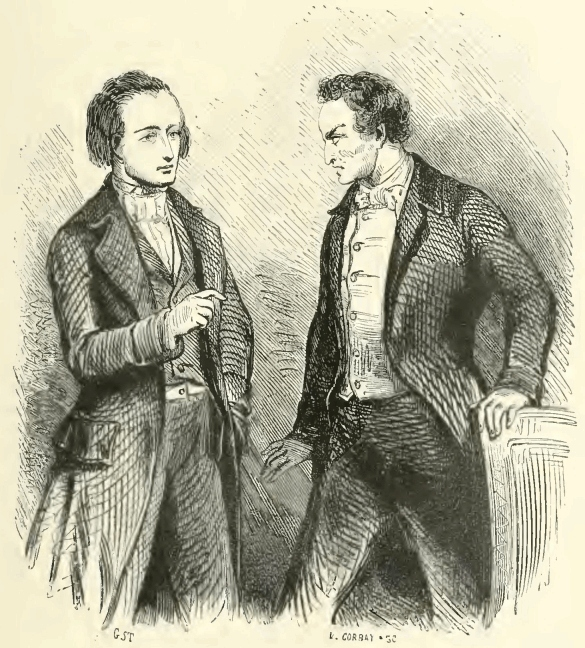
\includegraphics[width=\textwidth]{20277m.jpg}
\end{figure}

It was unexampled for a servant of the count’s to dare to dispute an
order of his, so the steward, without saying a word, followed his
master, who got into the carriage, and signed to him to follow, which
he did, taking his place respectfully on the front seat.
